\begin{pastexam}[label={px:nsysu-110-osds-01}]{中山資工所甲組 110 學年度 第 7 題}
（追蹤）

(10\%) Suppose that the preorder sequence of a binary tree is ABCDEFGH, and the inorder sequence is
ABDAFGHE. What is the postorder sequence of the binary tree ?
\end{pastexam}

\begin{pastsoln}
答案（採用中序 CBDAFGHE 的解讀）：後序是 \texttt{CDBHGFEA}。

\textbf{題目有錯}。 中序 ABDAFGHE 裡 A 出現兩次、C 沒有出現，不是 A--H 的排列，照字面沒有任何二元樹符合。 只改一個
字母、讓它變成合法中序的改法，是把兩個 A 之一改成 C：
\begin{itemize}
\item 第一個 A 改成 C：中序 \texttt{CBDAFGHE}；
\item 第二個 A 改成 C：中序 \texttt{ABDCFGHE}。
\end{itemize}
兩種都和前序 ABCDEFGH 配得起來。 第一種的樹左右都有子樹，比較像出題者想要的，下面以它為主，最後附上第二種的答案。
作答時要先寫出這個假設。

\textbf{重建}（資結書第~7.4~節）：前序的第一個是根；在中序裡找到根，左邊是左子樹、右邊是右子樹；左子樹有幾個
節點，前序裡根後面就取幾個給左子樹，遞迴下去。
\begin{itemize}
\item 前序 \texttt{ABCDEFGH}，根 A。 中序 \texttt{CBD | A | FGHE}：左子樹 $\{C, B, D\}$（$3$ 個），右子樹
$\{F, G, H, E\}$。 前序切成 \texttt{BCD} 和 \texttt{EFGH}。
\item 左子樹：前序 \texttt{BCD}，根 B；中序 \texttt{C | B | D}，C 是左子節點、D 是右子節點。
\item 右子樹：前序 \texttt{EFGH}，根 E；中序 \texttt{FGH | E |}，右邊是空的，F、G、H 都在左子樹。
\item E 的左子樹：前序 \texttt{FGH}，根 F；中序 \texttt{| F | GH}，左邊空，右子樹 \texttt{GH}。 前序 \texttt{GH}、
中序 \texttt{GH}：根 G，H 是 G 的右子節點。
\end{itemize}
\begin{center}
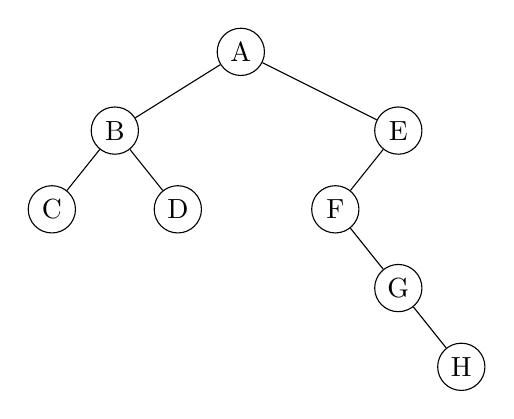
\begin{tikzpicture}[x=0.8cm,y=1.0cm,v/.style={circle,draw,inner sep=0pt,minimum size=6mm}]
\node[v] (A) at (3,0) {A};
\node[v] (B) at (1,-1) {B}; \node[v] (E) at (5.5,-1) {E};
\node[v] (C) at (0,-2) {C}; \node[v] (D) at (2,-2) {D}; \node[v] (F) at (4.5,-2) {F};
\node[v] (G) at (5.5,-3) {G};
\node[v] (H) at (6.5,-4) {H};
\draw (A)--(B) (A)--(E) (B)--(C) (B)--(D) (E)--(F) (F)--(G) (G)--(H);
\end{tikzpicture}
\end{center}
後序（左、右、根）：左子樹 B 的後序是 \texttt{CDB}；右子樹 E 的後序是 F 子樹的後序再接 E，F 子樹是 \texttt{HGF}，
所以是 \texttt{HGFE}；最後是根 A。 合起來：\texttt{CDBHGFEA}。

檢查：這棵樹的前序是 A, B, C, D, E, F, G, H，中序是 C, B, D, A, F, G, H, E，都和假設一致。

\textbf{另一種解讀}（中序 \texttt{ABDCFGHE}）：A 沒有左子樹，右子樹的根 B 也沒有左子樹；B 的右子樹根 C，左子節點 D，
右子樹 E（E 的左子樹是 F，F 的右子節點 G，G 的右子節點 H）。 後序是 \texttt{DHGFECBA}。
\end{pastsoln}
